%\subsection{Experiment design}
%    \label{subsection:Experiment_design}
%    %%Task description, stage 1 to 3 with survey
%    %\subsection{Experiment design}
%    \label{subsection:Experiment_design}
%    %%Task description, stage 1 to 3 with survey
%    %\subsection{Experiment design}
%    \label{subsection:Experiment_design}
%    %%Task description, stage 1 to 3 with survey
%    %\subsection{Experiment design}
%    \label{subsection:Experiment_design}
%    %%Task description, stage 1 to 3 with survey
%    \input{Text/ExperimentDesign}

With the VR system now comprehensively detailed, we transition into the experiment design phase, where we explore how this innovative virtual reality environment, equipped with the Computational Image Complexity Analysis (CICA) system-derived complexity data, will be utilized to investigate participants' responses to facade complexity variations.
This marks a pivotal stage in our study, where theory and technology converge to provide valuable insights into architectural complexity preferences.

The experiment is designed to comprehensively gauge participants' reactions to increasingly complex facade variations within immersive Virtual Reality simulations.
This process employs a Head-Mounted Display (HMD) and aims to quantitatively and qualitatively measure users' tolerance levels towards intricate facade designs (refer to Figure\ref{fig:ExperimentFlowchart}).

Conducted in our laboratory situated within the Architectural Environment Research Building, known as Building HE20, on the Itoshima campus of Kyushu University in Fukuoka, Japan, the experiment unfolds across three distinct stages: the `VR Interaction' stage, the `Screen-Based Ranking' stage, and the `Post-Experiment Survey' stage.



%!VR interaction stage

In the initial stage of the experiment, participants were introduced to a Virtual Reality simulation that faithfully replicated the actual laboratory and building where they were invited to take part (Figure\ref{fig:VRInteriorExterior}).
Within this immersive environment, participants faced a distinctive challenge.
Their task was to select the most comfortable facade variation from a range of options presented in the virtual setting.

This scenario presented an intriguing question: if the laboratory were to become their permanent workplace or study location, how would participants choose a facade that would enhance their daily experience of entering the building and working within its confines, making it more comfortable and engaging?.

Participants were granted the freedom to incorporate their personal preferences into their final decisions, with a primary emphasis on enhancing workplace comfort.
To address this facade design selection challenge, participants were tasked with evaluating and selecting their preferred facade from three distinct patterns, each featuring ten variations labeled by complexity level (see \ref{sec:AnnexVariations}).
These patterns were presented in a randomized order to ensure unbiased results and were easily accessible as separate stages through the VR interface.

To provide participants with a heightened sense of realism and immersion, a section of the laboratory was cleared to allow them to physically move around within the virtual simulation of the lab.
This enabled them to gain a deeper understanding of how each facade variation would impact their environment.

This stage of the experiment yielded valuable insights into participants' complexity tolerance levels, extracted from their recorded selections of the facade variations they found most comfortable.


%! Screen-based ranking stage

After the conclusion of each of the three pattern stages in the VR system, participants proceeded to the `Screen-Based Ranking' stage of the experiment.
The primary objective of this stage was to assess the accuracy of the `Computational Image Complexity Analysis' (CICA) system in evaluating the complexity of facade variations in comparison to the perceptions of the participants.

In this stage, participants were presented with the same set of 10 facade variations that had been processed by the CICA system.
However, this time, the presentation format shifted to a screen-based interface, and participants used a mouse and keyboard to navigate through the images of the facade variations.

Their task was to independently analyze these variations and arrange them according to their personal judgments of complexity.
Participants were specifically instructed to disregard any aesthetic preferences when ranking the facades and concentrate solely on the degree of complexity, arranging them from the least complex (level 1) to the most complex (level 10).
This stage of the experiment was repeated three times, once for each of the three patterns.
The responses from participants were meticulously recorded and later used for evaluating the alignment between the participants' ranking assessments and those generated by the CICA system.

The primary goal of this analysis was to ascertain if there existed any notable disparities between the CICA system's rankings and the perceptions of the participants.
By scrutinizing the results of this ranking comparison, the study aimed to refine the Complexity Tolerance Metric derived from the first stage, adjusting it based on the margin of error resulting from the deviation observed in the second stage.
This refined metric provides a more precise basis for forecasting future trends in architectural construction, facilitating informed conclusions.

%! Post-experiment survey stage

The third and final stage of the experiment, known as the `Post-interaction Survey' stage, takes place after participants have completed both the Facade design selection task in the `VR interaction stage' and the facade variation ranking task in the `Screen-based ranking stage' for all three patterns.
This survey comprises 15 questions categorized into two sections: `Participant Background' and `Complexity Perception.'

The survey, provided in detail in \ref{sec:Annexsurvey}, serves a dual purpose.
Firstly, it aims to gather insights into the participants' professional backgrounds, including any prior experience they may have in addressing facade design-related challenges.
Secondly, it seeks to understand participants' perceptions of complexity in building design, shedding light on the decision-making processes that underlie their choices during the experiment.

The `Background section' encompasses 5 multiple-choice questions designed to identify participants' professional backgrounds and their previous involvement in solving facade design problems.
In contrast, the `Complexity perception section' features 10 questions measured on a 7-point Likert scale.
These questions delve into participants' qualitative perceptions of complexity when assessing a building.
Additionally, they help identify the key factors that influence their selection of a particular facade variation.

%! Metrics purpose

In summary, the comprehensive design of our experiment, consisting of three distinct stages - the `VR Interaction' stage, the `Screen-Based Ranking' stage, and the `Post-Experiment Survey' stage, is aimed at providing a multifaceted understanding of user tolerance for complex facades and its implications for future construction trends.

By integrating the quantitative data from the VR system, the ranking comparisons from the screen-based stage, and the qualitative responses from the survey, we can form a comprehensive understanding of user tolerance for complex facades.
We can also identify the drivers behind participants' preferences, shedding light on the evolving trends in future construction.

This combined analysis positions us to answer the core research question: What degree of complexity within facade design, would users tolerate and accept for a building, and what insights do their preferences provide for future architectural trends?' By combining quantitative and qualitative findings, we aim to provide a nuanced perspective that contributes to the discourse on architectural complexity and its implications for contemporary design and construction.





With the VR system now comprehensively detailed, we transition into the experiment design phase, where we explore how this innovative virtual reality environment, equipped with the Computational Image Complexity Analysis (CICA) system-derived complexity data, will be utilized to investigate participants' responses to facade complexity variations.
This marks a pivotal stage in our study, where theory and technology converge to provide valuable insights into architectural complexity preferences.

The experiment is designed to comprehensively gauge participants' reactions to increasingly complex facade variations within immersive Virtual Reality simulations.
This process employs a Head-Mounted Display (HMD) and aims to quantitatively and qualitatively measure users' tolerance levels towards intricate facade designs (refer to Figure\ref{fig:ExperimentFlowchart}).

Conducted in our laboratory situated within the Architectural Environment Research Building, known as Building HE20, on the Itoshima campus of Kyushu University in Fukuoka, Japan, the experiment unfolds across three distinct stages: the `VR Interaction' stage, the `Screen-Based Ranking' stage, and the `Post-Experiment Survey' stage.



%!VR interaction stage

In the initial stage of the experiment, participants were introduced to a Virtual Reality simulation that faithfully replicated the actual laboratory and building where they were invited to take part (Figure\ref{fig:VRInteriorExterior}).
Within this immersive environment, participants faced a distinctive challenge.
Their task was to select the most comfortable facade variation from a range of options presented in the virtual setting.

This scenario presented an intriguing question: if the laboratory were to become their permanent workplace or study location, how would participants choose a facade that would enhance their daily experience of entering the building and working within its confines, making it more comfortable and engaging?.

Participants were granted the freedom to incorporate their personal preferences into their final decisions, with a primary emphasis on enhancing workplace comfort.
To address this facade design selection challenge, participants were tasked with evaluating and selecting their preferred facade from three distinct patterns, each featuring ten variations labeled by complexity level (see \ref{sec:AnnexVariations}).
These patterns were presented in a randomized order to ensure unbiased results and were easily accessible as separate stages through the VR interface.

To provide participants with a heightened sense of realism and immersion, a section of the laboratory was cleared to allow them to physically move around within the virtual simulation of the lab.
This enabled them to gain a deeper understanding of how each facade variation would impact their environment.

This stage of the experiment yielded valuable insights into participants' complexity tolerance levels, extracted from their recorded selections of the facade variations they found most comfortable.


%! Screen-based ranking stage

After the conclusion of each of the three pattern stages in the VR system, participants proceeded to the `Screen-Based Ranking' stage of the experiment.
The primary objective of this stage was to assess the accuracy of the `Computational Image Complexity Analysis' (CICA) system in evaluating the complexity of facade variations in comparison to the perceptions of the participants.

In this stage, participants were presented with the same set of 10 facade variations that had been processed by the CICA system.
However, this time, the presentation format shifted to a screen-based interface, and participants used a mouse and keyboard to navigate through the images of the facade variations.

Their task was to independently analyze these variations and arrange them according to their personal judgments of complexity.
Participants were specifically instructed to disregard any aesthetic preferences when ranking the facades and concentrate solely on the degree of complexity, arranging them from the least complex (level 1) to the most complex (level 10).
This stage of the experiment was repeated three times, once for each of the three patterns.
The responses from participants were meticulously recorded and later used for evaluating the alignment between the participants' ranking assessments and those generated by the CICA system.

The primary goal of this analysis was to ascertain if there existed any notable disparities between the CICA system's rankings and the perceptions of the participants.
By scrutinizing the results of this ranking comparison, the study aimed to refine the Complexity Tolerance Metric derived from the first stage, adjusting it based on the margin of error resulting from the deviation observed in the second stage.
This refined metric provides a more precise basis for forecasting future trends in architectural construction, facilitating informed conclusions.

%! Post-experiment survey stage

The third and final stage of the experiment, known as the `Post-interaction Survey' stage, takes place after participants have completed both the Facade design selection task in the `VR interaction stage' and the facade variation ranking task in the `Screen-based ranking stage' for all three patterns.
This survey comprises 15 questions categorized into two sections: `Participant Background' and `Complexity Perception.'

The survey, provided in detail in \ref{sec:Annexsurvey}, serves a dual purpose.
Firstly, it aims to gather insights into the participants' professional backgrounds, including any prior experience they may have in addressing facade design-related challenges.
Secondly, it seeks to understand participants' perceptions of complexity in building design, shedding light on the decision-making processes that underlie their choices during the experiment.

The `Background section' encompasses 5 multiple-choice questions designed to identify participants' professional backgrounds and their previous involvement in solving facade design problems.
In contrast, the `Complexity perception section' features 10 questions measured on a 7-point Likert scale.
These questions delve into participants' qualitative perceptions of complexity when assessing a building.
Additionally, they help identify the key factors that influence their selection of a particular facade variation.

%! Metrics purpose

In summary, the comprehensive design of our experiment, consisting of three distinct stages - the `VR Interaction' stage, the `Screen-Based Ranking' stage, and the `Post-Experiment Survey' stage, is aimed at providing a multifaceted understanding of user tolerance for complex facades and its implications for future construction trends.

By integrating the quantitative data from the VR system, the ranking comparisons from the screen-based stage, and the qualitative responses from the survey, we can form a comprehensive understanding of user tolerance for complex facades.
We can also identify the drivers behind participants' preferences, shedding light on the evolving trends in future construction.

This combined analysis positions us to answer the core research question: What degree of complexity within facade design, would users tolerate and accept for a building, and what insights do their preferences provide for future architectural trends?' By combining quantitative and qualitative findings, we aim to provide a nuanced perspective that contributes to the discourse on architectural complexity and its implications for contemporary design and construction.





With the VR system now comprehensively detailed, we transition into the experiment design phase, where we explore how this innovative virtual reality environment, equipped with the Computational Image Complexity Analysis (CICA) system-derived complexity data, will be utilized to investigate participants' responses to facade complexity variations.
This marks a pivotal stage in our study, where theory and technology converge to provide valuable insights into architectural complexity preferences.

The experiment is designed to comprehensively gauge participants' reactions to increasingly complex facade variations within immersive Virtual Reality simulations.
This process employs a Head-Mounted Display (HMD) and aims to quantitatively and qualitatively measure users' tolerance levels towards intricate facade designs (refer to Figure\ref{fig:ExperimentFlowchart}).

Conducted in our laboratory situated within the Architectural Environment Research Building, known as Building HE20, on the Itoshima campus of Kyushu University in Fukuoka, Japan, the experiment unfolds across three distinct stages: the `VR Interaction' stage, the `Screen-Based Ranking' stage, and the `Post-Experiment Survey' stage.



%!VR interaction stage

In the initial stage of the experiment, participants were introduced to a Virtual Reality simulation that faithfully replicated the actual laboratory and building where they were invited to take part (Figure\ref{fig:VRInteriorExterior}).
Within this immersive environment, participants faced a distinctive challenge.
Their task was to select the most comfortable facade variation from a range of options presented in the virtual setting.

This scenario presented an intriguing question: if the laboratory were to become their permanent workplace or study location, how would participants choose a facade that would enhance their daily experience of entering the building and working within its confines, making it more comfortable and engaging?.

Participants were granted the freedom to incorporate their personal preferences into their final decisions, with a primary emphasis on enhancing workplace comfort.
To address this facade design selection challenge, participants were tasked with evaluating and selecting their preferred facade from three distinct patterns, each featuring ten variations labeled by complexity level (see \ref{sec:AnnexVariations}).
These patterns were presented in a randomized order to ensure unbiased results and were easily accessible as separate stages through the VR interface.

To provide participants with a heightened sense of realism and immersion, a section of the laboratory was cleared to allow them to physically move around within the virtual simulation of the lab.
This enabled them to gain a deeper understanding of how each facade variation would impact their environment.

This stage of the experiment yielded valuable insights into participants' complexity tolerance levels, extracted from their recorded selections of the facade variations they found most comfortable.


%! Screen-based ranking stage

After the conclusion of each of the three pattern stages in the VR system, participants proceeded to the `Screen-Based Ranking' stage of the experiment.
The primary objective of this stage was to assess the accuracy of the `Computational Image Complexity Analysis' (CICA) system in evaluating the complexity of facade variations in comparison to the perceptions of the participants.

In this stage, participants were presented with the same set of 10 facade variations that had been processed by the CICA system.
However, this time, the presentation format shifted to a screen-based interface, and participants used a mouse and keyboard to navigate through the images of the facade variations.

Their task was to independently analyze these variations and arrange them according to their personal judgments of complexity.
Participants were specifically instructed to disregard any aesthetic preferences when ranking the facades and concentrate solely on the degree of complexity, arranging them from the least complex (level 1) to the most complex (level 10).
This stage of the experiment was repeated three times, once for each of the three patterns.
The responses from participants were meticulously recorded and later used for evaluating the alignment between the participants' ranking assessments and those generated by the CICA system.

The primary goal of this analysis was to ascertain if there existed any notable disparities between the CICA system's rankings and the perceptions of the participants.
By scrutinizing the results of this ranking comparison, the study aimed to refine the Complexity Tolerance Metric derived from the first stage, adjusting it based on the margin of error resulting from the deviation observed in the second stage.
This refined metric provides a more precise basis for forecasting future trends in architectural construction, facilitating informed conclusions.

%! Post-experiment survey stage

The third and final stage of the experiment, known as the `Post-interaction Survey' stage, takes place after participants have completed both the Facade design selection task in the `VR interaction stage' and the facade variation ranking task in the `Screen-based ranking stage' for all three patterns.
This survey comprises 15 questions categorized into two sections: `Participant Background' and `Complexity Perception.'

The survey, provided in detail in \ref{sec:Annexsurvey}, serves a dual purpose.
Firstly, it aims to gather insights into the participants' professional backgrounds, including any prior experience they may have in addressing facade design-related challenges.
Secondly, it seeks to understand participants' perceptions of complexity in building design, shedding light on the decision-making processes that underlie their choices during the experiment.

The `Background section' encompasses 5 multiple-choice questions designed to identify participants' professional backgrounds and their previous involvement in solving facade design problems.
In contrast, the `Complexity perception section' features 10 questions measured on a 7-point Likert scale.
These questions delve into participants' qualitative perceptions of complexity when assessing a building.
Additionally, they help identify the key factors that influence their selection of a particular facade variation.

%! Metrics purpose

In summary, the comprehensive design of our experiment, consisting of three distinct stages - the `VR Interaction' stage, the `Screen-Based Ranking' stage, and the `Post-Experiment Survey' stage, is aimed at providing a multifaceted understanding of user tolerance for complex facades and its implications for future construction trends.

By integrating the quantitative data from the VR system, the ranking comparisons from the screen-based stage, and the qualitative responses from the survey, we can form a comprehensive understanding of user tolerance for complex facades.
We can also identify the drivers behind participants' preferences, shedding light on the evolving trends in future construction.

This combined analysis positions us to answer the core research question: What degree of complexity within facade design, would users tolerate and accept for a building, and what insights do their preferences provide for future architectural trends?' By combining quantitative and qualitative findings, we aim to provide a nuanced perspective that contributes to the discourse on architectural complexity and its implications for contemporary design and construction.





The experiment is designed to comprehensively measure the response of participant to increasingly complex facade variations through Virtual Reality (VR) simulations using a Heads-Up mounted display Heads mo Display (HUD) on the decision-making to quantitatively and qualitatively measure the level of tolerance of users of a building to complex envelop design (see Figure\ref{fig:ExperimentFlowchart}).

It consists of three distinct stages: the `VR interaction' stage, the `Screen-based ranking' stage, and the `Post-experiment Survey' stage.

%% Figure Experiment Design flowchart
    \begin{figure}[htb]
      \centering
      % trim=left 190 down 250 right 150 top5
      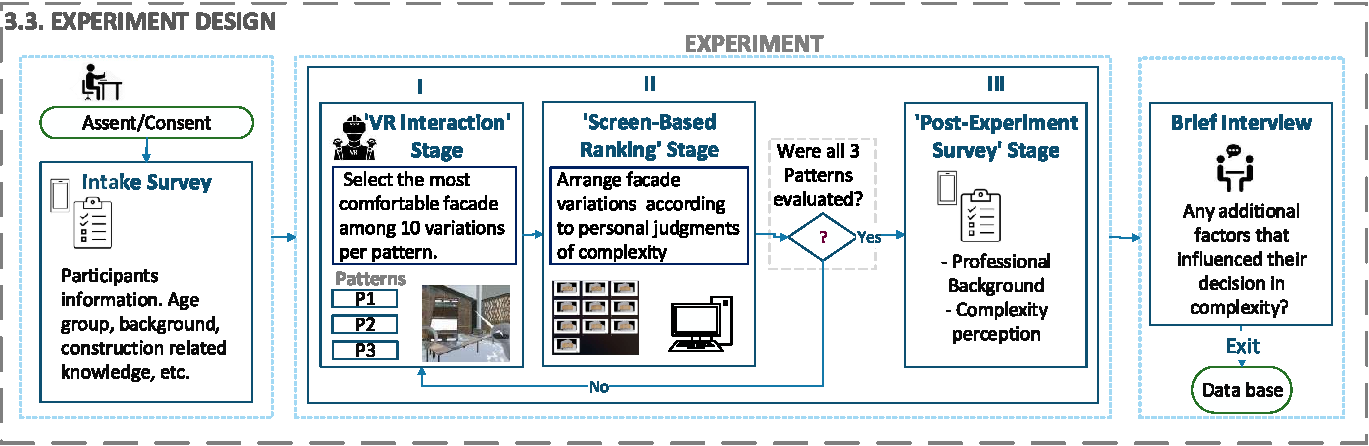
\includegraphics[width= \linewidth, trim=0 0 0 0, clip]{Images/FlowchartExperiment}
      \caption{Flowchart illustrating the Experiment design stages, depicting the VR interaction stage, the Screen-based ranking stage and the Post-experiment survey.}
      \label{fig:ExperimentFlowchart}
    \end{figure}